\documentclass[tikz,border=4pt]{standalone}
\usepackage[T1]{fontenc}
\usepackage{lmodern}
\usetikzlibrary{arrows.meta,positioning,fit,backgrounds,calc}
\begin{document}
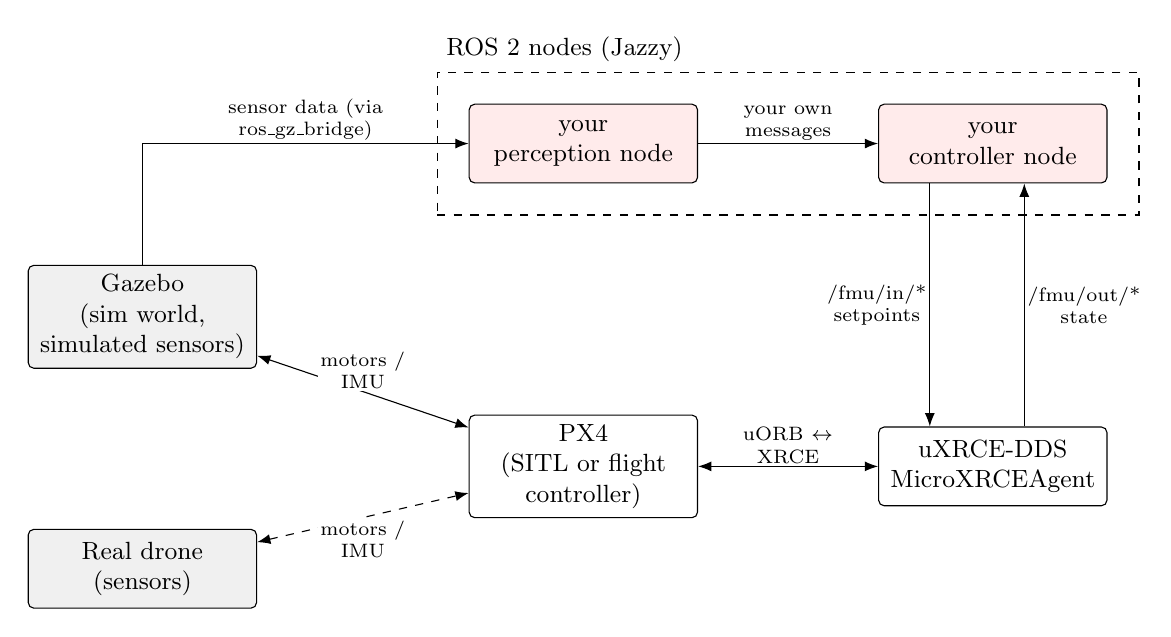
\begin{tikzpicture}[
  blk/.style={draw,rounded corners=2pt,minimum height=10mm,minimum width=29mm,align=center,font=\small,fill=white},
  ros/.style={blk,fill=red!8},
  ext/.style={blk,fill=gray!12},
  lab/.style={font=\scriptsize,fill=white,inner sep=1pt,align=center},
  >={Latex}]
\node[ext] (gz) at (0,0.4) {Gazebo\\(sim world,\\simulated sensors)};
\node[ext] (real) at (0,-2.8) {Real drone\\(sensors)};
\node[blk] (px4) at (5.6,-1.5) {PX4\\(SITL or flight\\controller)};
\node[blk] (dds) at (10.8,-1.5) {uXRCE-DDS\\MicroXRCEAgent};
\node[ros] (per) at (5.6,2.6) {your\\perception node};
\node[ros] (ctl) at (10.8,2.6) {your\\controller node};
\begin{scope}[on background layer]
\node[draw,dashed,inner sep=4mm,fit=(per)(ctl)] (rosbox) {};
\end{scope}
\node[font=\small,anchor=south west] at (rosbox.north west) {ROS 2 nodes (Jazzy)};
\draw[<->] (gz) -- node[lab,above]{motors /\\IMU} (px4);
\draw[<->,dashed] (real) -- node[lab,below]{motors /\\IMU} (px4);
\draw[<->] (px4) -- node[lab,above]{uORB $\leftrightarrow$\\XRCE} (dds);
\draw[->] (gz.north) |- node[lab,pos=0.75,above]{sensor data (via\\ros\_gz\_bridge)} (per.west);
\draw[->] (per) -- node[lab,above]{your own\\messages} (ctl);
\draw[->] ($(dds.north)+(4mm,0)$) -- node[lab,right,pos=0.5]{/fmu/out/*\\state} ($(ctl.south)+(4mm,0)$);
\draw[->] ($(ctl.south)+(-8mm,0)$) -- node[lab,left,pos=0.5]{/fmu/in/*\\setpoints} ($(dds.north)+(-8mm,0)$);
\end{tikzpicture}
\end{document}
